%!TEX root = ../../../super_main.tex

\section{About Page}
\label{sec:about_page}

We have implemented an about page, with a simple layout, in the \launcher settings in order to properly give credit to the open source projects used in the \launcher, and thereby in the entire \giraf application suite because of the shared content provider in the \launcher. This was requested by group \emph{SW610F15} (the database subproject product owner). The about page can be seen in \figref{fig:about_page}.
\\\\
Notice that the icon used for the about-tab could be changed to something different than the general-tab, for instance an information ``i''. However, no icons have been added for this use-case, so a last-minute solution was implemented. Ideally a new icon should be designed, implemented and described in the design manual.

\begin{figure}[!htbp]
	\centering
	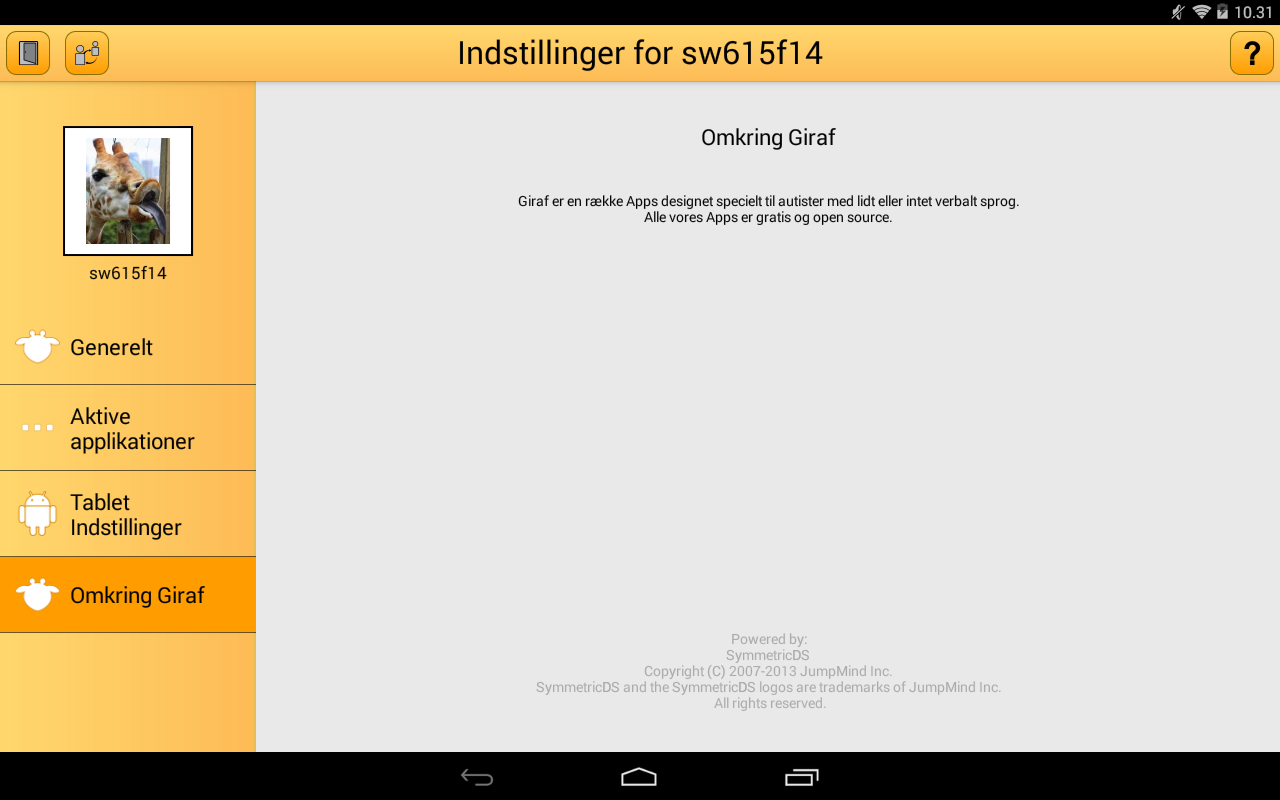
\includegraphics[width=\textwidth]{sprint_four/about_page}
	\caption{About page}
	\label{fig:about_page}
\end{figure}
